
%% start of file `cv_german.tex', based on `template_en.tex` by Xavier Danaux (xdanaux@gmail.com).
% This work may be distributed and/or modified under the
% conditions of the LaTeX Project Public License version 1.3c,
% available at http://www.latex-project.org/lppl/.
% 
% Thomas Quaritsch <t.quaritsch@student.tugraz.at>

\documentclass[11pt,a4paper]{moderncv}

\usepackage[german]{babel}
\usepackage{moderncv-additions}

% moderncv themes
\moderncvtheme{casual} % optional arguments are 'blue' (default), 'orange', 'red', 'green', 'grey' and 'roman' (for roman fonts, instead of sans serif fonts)
%\moderncvtheme[green]{classic}                % idem

% character encoding
\usepackage[utf8]{inputenc}                   % replace by the encoding you are using

% adjust the page margins
\usepackage[scale=0.8]{geometry}
\setlength{\hintscolumnwidth}{3cm}			  % if you want to change the width of the column with the dates
%\AtBeginDocument{\setlength{\maketitlenamewidth}{6cm}}  % only for the classic theme, if you want to change the width of your name placeholder (to leave more space for your address details

\AtBeginDocument{\recomputelengths}           % required when changes are made to page layout lengths

% personal data
\firstname{Max}
\familyname{Mustermann}
%\title{Resumé title (optional)}               % optional, remove the line if not wanted
\address{Musterstr. 1}{12345 Stuttgart}        % optional, remove the line if not wanted
\mobile{+49 123 4567891}                     % optional, remove the line if not wanted
%\phone{phone (optional)}                      % optional, remove the line if not wanted
%\fax{fax (optional)}                          % optional, remove the line if not wanted
\email{max\_mustermann@outlook.com}                      % optional, remove the line if not wanted
%\extrainfo{additional information (optional)} % optional, remove the line if not wanted
%\photo[64pt]{foto}                          % '64pt' is the height the picture must be resized to and 'picture' is the name of the picture file; optional, remove the line if not wanted
%\quote{``Das ist ein toller Frusterspruch\\ von Friede Frusterfrau.'' -- Friede Frusterfrau}                 % optional, remove the line if not wanted

%\nopagenumbers{}                             % uncomment to suppress automatic page numbering for CVs longer than one page

\graphicspath{{../attachments/}}


%The doit command will break lines within the cventry arguments
\newcommand{\doit}{\newline} %uncomment if linebreak in \cventry
%\newcommand{\doit}{} %uncomment if NO linebreak in \cventry


%----------------------------------------------------------------------------------
%            content
%----------------------------------------------------------------------------------

\begin{document}

% color redefinitions must be after \begin{document}!
\definecolor{firstnamecolor}{RGB}{0,0,0}
\definecolor{familynamecolor}{RGB}{0,0,0}
\definecolor{quotecolor}{RGB}{125,85,85}
\definecolor{addresscolor}{RGB}{100,100,100}
\definecolor{sectionrectanglecolor}{RGB}{139,0,0}
\definecolor{sectiontitlecolor}{RGB}{139,0,0}
\definecolor{subsectioncolor}{RGB}{50,50,50}
\definecolor{footersymbolcolor}{RGB}{50,50,50}	

\makeatletter

\pagestyle{empty}
\chapter*{Bewerbungs}{unterlagen}

\vspace*{50mm}
\begin{minipage}{\textwidth}
	\vspace*{3mm}
	\familynamestyle{\@firstname}~~\firstnamestyle{\@familyname} 	
	\hspace*{15mm}{{\color{firstnamecolor}
\includegraphics[width=175pt]{foto}}}\\[3mm]
	\@addressstreet, \@addresscity ~~~ \mobilesymbol~\@mobile ~~~ \emailsymbol~\@email
\end{minipage}
\begin{minipage}{70pt}
	
\end{minipage}

\vfill

\begin{minipage}{1.0\textwidth}
	\section{Inhalt}
	\tableofcontents
\end{minipage}

\newpage
\pagestyle{fancy}
\chapter{Curriculum}{~Vit\ae}
\makequote

\section{Persönliche Daten}
%%%%%%%%%%%%%%%%%%%%%%%%%%%%%%%%%%%%%%%%%%%%%%%%%%%%%%%%%%%%%%%%%%%%
\cvline{Name}{\@firstname~\@familyname}
\cvline{Anschrift}{\@addressstreet, \@addresscity}
\cvline{Telefon}{\@mobile}
\cvline{E-Mail}{\@email}
\cvline{Geburtsdaten}{1. Januar 1990 in Stuttgart}
%\cvline{Staatsbürgerschaft}{Deutschland}
\cvline{Familienstand}{ledig}
%\cvline{Präsenzdienst}{abgeleistet}
%\cvline{Führerschein}{A,B,C,D,E,F,G}
\makeatother 

%\cventry{year--year}{Degree}{Institution}{City}{\textit{Grade}}{Description}  % arguments 3 to 6 are optional

\section{Ausbildung} 
%%%%%%%%%%%%%%%%%%%%%%%%%%%%%%%%%%%%%%%%%%%%%%%%%%%%%%%%%%%%%%%%%%%%

\cventry{00/2015 -- 00/2016}
{Master of Science Musterstudium}
{\doit Muster Hochschule/Universität}
{\doit {Note Studium: 1,5 | Note Thesis: 1,0}}
{\doit Thesentitel: Entwicklung von noch viel mehr Mustermethoden zum Mustern von Mustersystemen}
{}  % arguments 3 to 6 are optional

\cventry{00/2010 -- 00/2015}
{Bachelor of Science Musterstudium}
{\doit Muster Hochschule/Universität}
{\doit Note Studium: 2,0 | Note Thesis: 1,3}
{\doit Vertiefung: Mustervertiefung,
\doit Thesentitel: Entwicklung von Mustermethoden zum Mustern von Mustersystemen}
{}  % arguments 3 to 6 are optional



\cventry{(00/09 - 00/10)}
{Zivildienst}
{Muster\&Muster GmbH}
{\doit {Betreuung von Schwerbehinderten | \glqq Essen auf Rädern\grqq{}}}
{}
{}  % arguments 3 to 6 are optional

\cventry{00/2006 -- 00/2009}
{Ausbildung zum Musterkaufmann/Mustermechaniker ODER Abitur}
{\doit Musterbetrieb A\&B AG}
{\doit {Note Ausbildung: 1,8}}
{}
{}  % arguments 3 to 6 are optional

\section{Auslandsstudium}	
%%%%%%%%%%%%%%%%%%%%%%%%%%%%%%%%%%%%%%%%%%%%%%%%%%%%%%%%%%%%%%%%%%%%
\cventry{08/2013 -- 12/2013}
{University Fancy-Pants, Schottland}
{\doit Auslandssemester Musterstudium}
{PROMOS-Stipendium}
{\doit Studieninhalte: Computer-aided engineering | Regelungstechnik | Muster}
{}  % arguments 3 to 6 are optional

\section{Berufserfahrung} 
%%%%%%%%%%%%%%%%%%%%%%%%%%%%%%%%%%%%%%%%%%%%%%%%%%%%%%%%%%%%%%%%%%%%
\cventry{00/2016 -- 00/2016}{Institut für Angewandte Forschung der Muster Hochschule}
{\doit Wissenschaftlicher Mitarbeiter am BMBF-Projekt \glqq Muster\grqq{}}
{\doit Musterarbeitsinhalte in Kurzform. Lorem ipsum dolor sit amet, consetetur sadipscing elitr, sed diam nonumy eirmod tempor invidunt ut labore et dolore magna aliquyam erat, sed diam voluptua. At vero eos et accusam et justo duo dolores et ea rebum. Stet clita kasd gubergren, no sea takimata sanctus est Lorem ipsum dolor sit amet}
{}
{}  % arguments 3 to 6 are optional

\cventry{00/2014 -- 00/2014}{Muster Group - Musterstadt}
{\doit Praxissemester im Forschungs- und Innovationszentrum}
{\doit Inhalte in 2 Zeilen. Lorem ipsum dolor sit amet, consetetur sadipscing elitr, sed diam nonumy eirmod}
{Optimierung bestehender Mustertools}
{}  % arguments 3 to 6 are optional

\cventry{07/2010 -- 08/2010}
{Muster\&Co GmbH - Mustertal}
{\doit Technisches Vorpraktikum}
{\doit Grundlagen der Metallbearbeitung}
{Manuelle und maschinelle Bearbeitungsverfahren}
{}  % arguments 3 to 6 are optional



%\section{Sprachen} 
%%%%%%%%%%%%%%%%%%%%%%%%%%%%%%%%%%%%%%%%%%%%%%%%%%%%%%%%%%%%%%%%%%%%%
%
%\cvline{Deutsch}{Muttersprache}{}
%\cvline{Englisch}{Verstehen A1, Sprechen B2, Schreiben C3 \hfill {\scriptsize \itshape Europäische Kompetenzstufe}}

\section{Weitere Qualifikationen} 
%%%%%%%%%%%%%%%%%%%%%%%%%%%%%%%%%%%%%%%%%%%%%%%%%%%%%%%%%%%%%%%%%%%%

\cvline{Sprachen}
{Deutsch: Muttersprache\newline
Englisch: Verhandlungssicher (C1)\hfill {\scriptsize \itshape Europäische Kompetenzstufe}}

\cvline{CAD-Systeme}
{Autodesk Inventor\hfill {\scriptsize \itshape sehr gute Kenntnisse}\newline
PTC Creo (vormals: Pro/Engineer)\hfill {\scriptsize \itshape gute Kenntnisse}}

\cvline{Betriebl. Software}
{SAP R/3\hfill {\scriptsize \itshape Grundkenntnisse}}

\cvline{Programmiersprachen}
{Objektorientiert: Java\hfill {\scriptsize \itshape gute Kenntnisse}\newline
Skriptsprachen: Shell-Script, YAML, VBA\hfill {\scriptsize \itshape gute Kenntnisse}\newline
Webtechnologien: HTML, CSS, XML\hfill {\scriptsize \itshape gute Kenntnisse}}

\cvline{Virtualisierung}
{Virtuelle Maschine: VirtualBox, Vagrant\hfill {\scriptsize \itshape sehr gute Kenntnisse}\newline
Container: Docker  --  Containernetzwerk: Weave\hfill {\scriptsize \itshape sehr gute Kenntnisse}}

\cvline{Clustermanagement}
{Kubernetes \hfill {\scriptsize \itshape gute Kenntnisse}\newline
Apache Ambari \hfill {\scriptsize \itshape gute Kenntnisse}\newline}

\cvline{Office / Textverarbeitung}
{Microsoft Office\hfill {\scriptsize \itshape sehr gute Kenntnisse}\newline
LaTex\hfill {\scriptsize \itshape gute Kenntnisse}\newline}




\section{Sonstiges} 
%%%%%%%%%%%%%%%%%%%%%%%%%%%%%%%%%%%%%%%%%%%%%%%%%%%%%%%%%%%%%%%%%%%%

\cvline{Interessen}
{Fußball, Skifahren, Lesen, Kochen}


Stuttgart, den 01.01.2017 ~~~~~~~~~~~ 
\includegraphics[height=0.035\textheight]{signature.png}

%\newpage
%
%\section{Außeruniversitäre Tätigkeiten} 
%%%%%%%%%%%%%%%%%%%%%%%%%%%%%%%%%%%%%%%%%%%%%%%%%%%%%%%%%%%%%%%%%%%%%
%
%\cvline{....}{....}
%
%\section{Interessen}
%%%%%%%%%%%%%%%%%%%%%%%%%%%%%%%%%%%%%%%%%%%%%%%%%%%%%%%%%%%%%%%%%%%%%
%
%\cvline{....}{....}
%
%\section{Publikationen} 
%%%%%%%%%%%%%%%%%%%%%%%%%%%%%%%%%%%%%%%%%%%%%%%%%%%%%%%%%%%%%%%%%%%%%
%
%\subsection{Konferenzen und Workshops}
%
%\cvline{mm/jjjj}{Autor 1 und Autor 2. \textbf{Mustertitel: Unser tolles Paper.} In \textit{Proceedings of the First Muster Workshop 1970}, Musterstadt, Musterland, YYYY.}
%
%% \newpage
%
%\subsection{Technical Reports}
%
%\cvline{....}{....}
%
%\cvline{....}{alternativ kann man auch BibTex verwenden:}
%
%\renewcommand*{\refname}{Abschlussarbeiten}
%\nocite{*}
%\bibliographystyle{cv}
%\bibliography{publications}       % 'publications' is the name of a BibTeX file

\newpage
\chapter{Arbeits}{zeugnis}
\vspace*{1cm}
\begin{center}
	 \fbox{
\includegraphics[height=0.85\textheight]{Arbeitszeugnis.pdf}}	
\end{center}

\newpage
\chapter{Master}{zeugnis}
\vspace*{1cm}
\begin{center}
	 \fbox{
\includegraphics[height=0.85\textheight]{Masterzeugnis-1.pdf}}	
\end{center}

\newpage
\chapter*{Master}{zeugnis}
\vspace*{1cm}
\begin{center}
	 \fbox{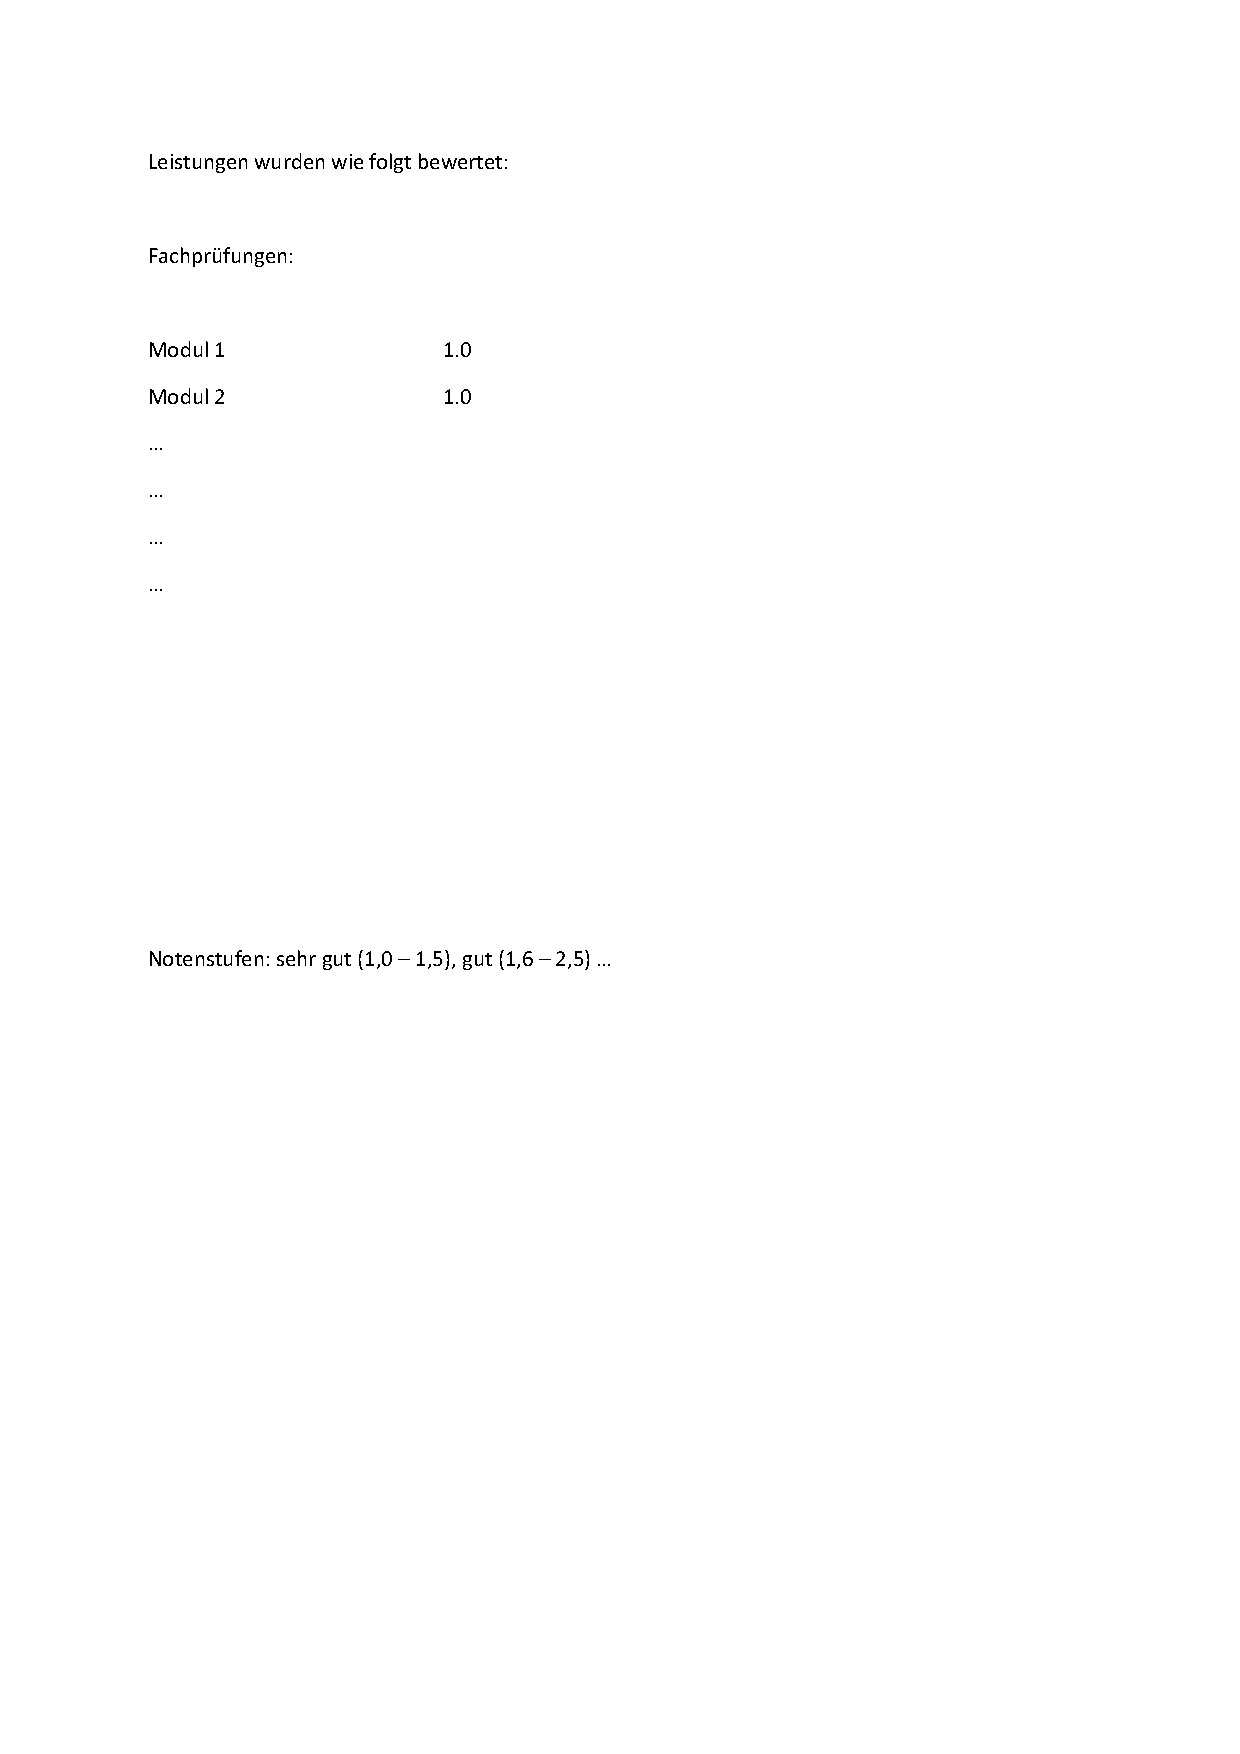
\includegraphics[height=0.85\textheight]{Masterzeugnis-2.pdf}}	
\end{center}


\newpage
\chapter{Bachelor}{zeugnis}
\vspace*{1cm}
\begin{center}
	 \fbox{
\includegraphics[height=0.85\textheight]{Bachelorzeugnis-1.pdf}}	
\end{center}

\newpage
\chapter*{Bachelor}{zeugnis}
\vspace*{1cm}
\begin{center}
	 \fbox{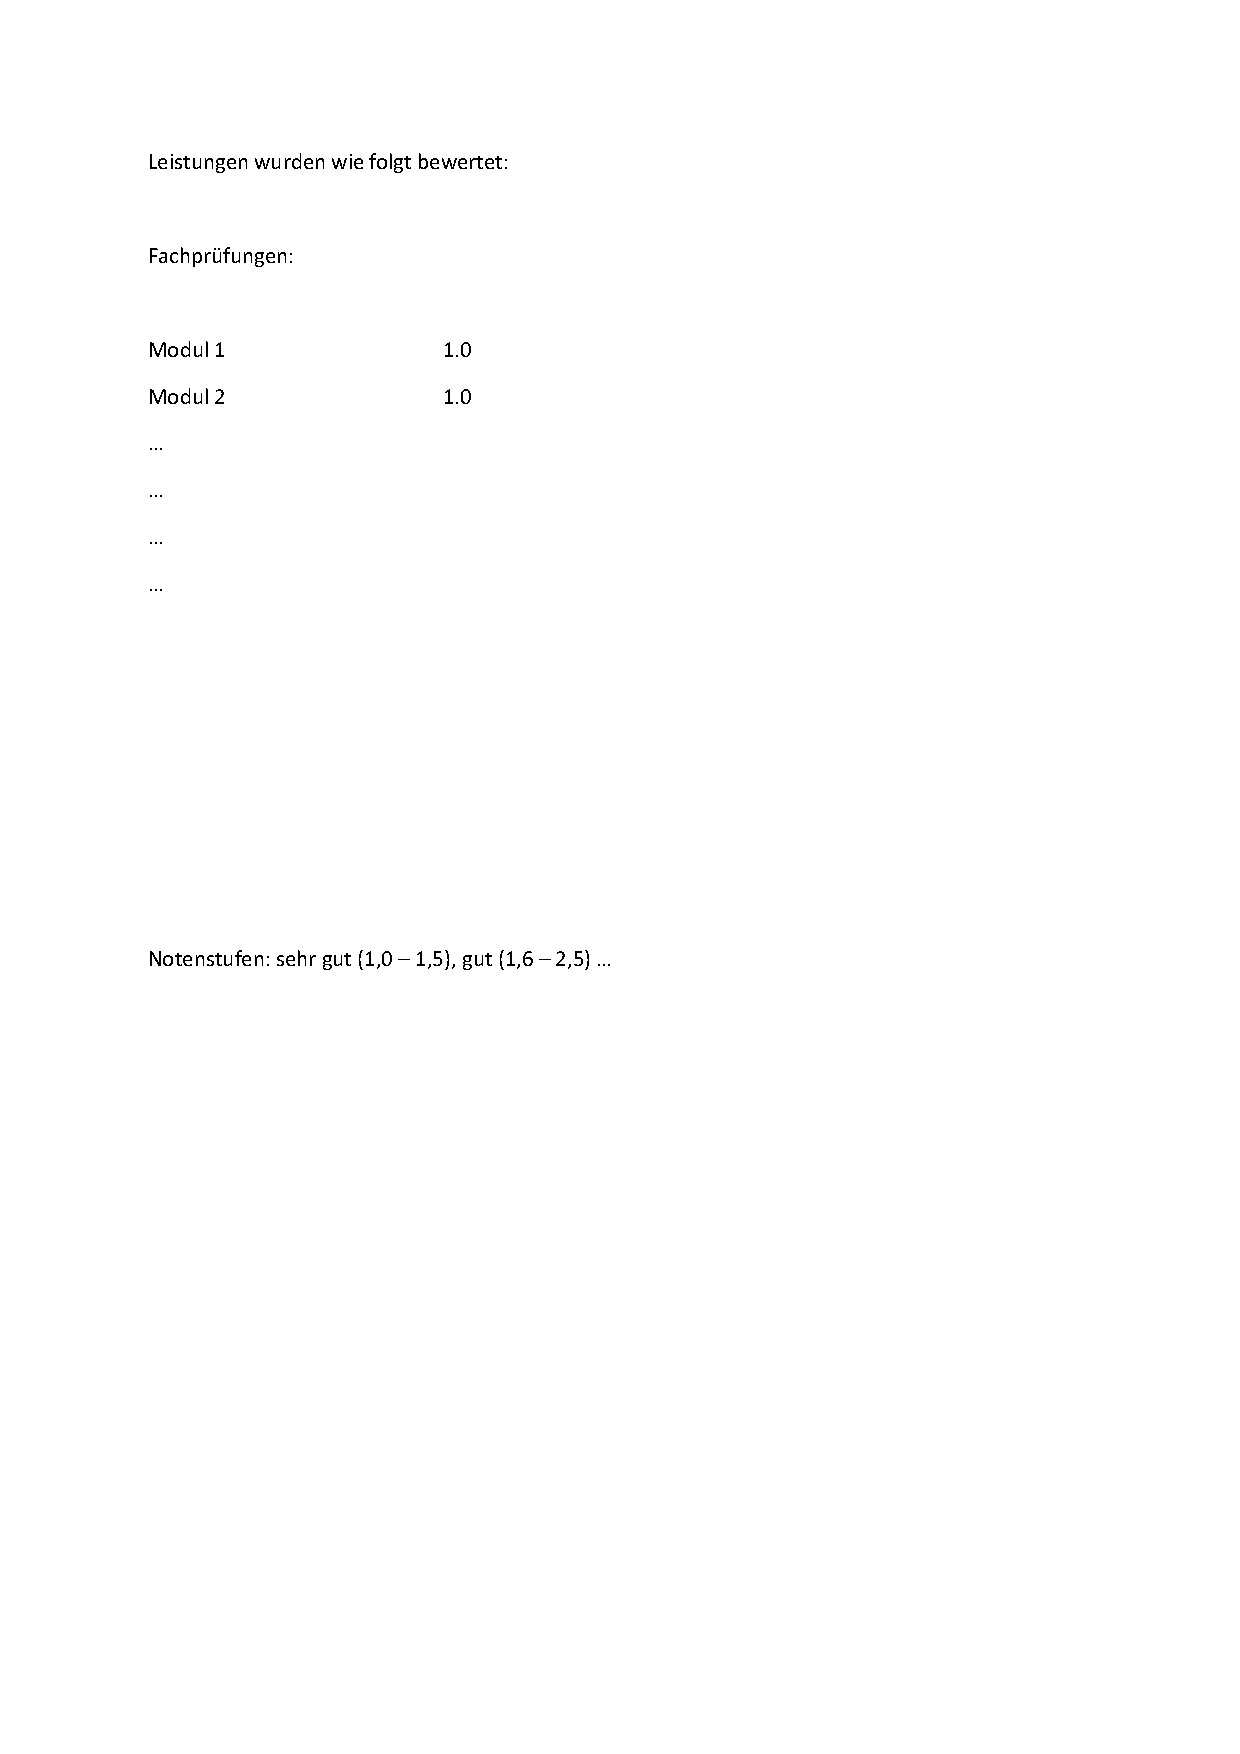
\includegraphics[height=0.85\textheight]{Masterzeugnis-2.pdf}}	
\end{center}


\end{document}

% end of file `cv_german.tex'
